\section{PPF and Flux Study}
Equation \ref{eq:reaction-rate-fission} shows the relationship between fission reaction rate, 
flux, and material properties. 
\begin{align}
\label{eq:reaction-rate-fission}
    RR_f &= \Phi \times \sigma_f \times N \\
\intertext{where}
    RR_f &= \mbox{fission reaction rate } [reactions \cdot cm^{-3} \cdot s^{-1}]\nonumber \\
    \Phi &= \mbox{neutron flux } [neutrons \cdot cm^{-2} \cdot s^{-1}] \nonumber \\
    \sigma_f &= \mbox{microscopic cross section } [cm^2] \nonumber \\
    N &= \mbox{atomic number density } [atoms \cdot cm^{-3}] \nonumber 
\end{align}

Since microscopic cross section is constant for the same fuel material, we can rearrange 
Equation \ref{eq:reaction-rate-fission} into Equation \ref{eq:reaction-rate-fission-prop}: 
\begin{align}
    \label{eq:reaction-rate-fission-prop}
    \Phi \propto \frac{RR_f}{N}
    \intertext{where}
    \Phi &= \mbox{neutron flux } [neutrons \cdot cm^{-2} \cdot s^{-1}] \nonumber \\
    RR_f &= \mbox{fission reaction rate } [reactions \cdot cm^{-3} \cdot s^{-1}]\nonumber \\
    N &= \mbox{atomic number density } [atoms \cdot cm^{-3}] \nonumber
\end{align}
In Section \ref{sec:ahtr_slab_output}, I defined $PPF_{fuel}$ as: 
\begin{align}
    PPF_{fuel} &= max(\frac{fqr_j}{PF_j}) \div ave(\frac{fqr_j}{PF_j})
\intertext{where}
j &= \mbox{discretized fuel area j} \nonumber \\
PPF_{fuel} &= \mbox{fuel-normalized power peaking factor} \nonumber \\
fqr_j &= \mbox{fission-q-recoverable at position j} \nonumber \\
PF_j &= \mbox{fuel packing fraction at position j} \nonumber
\end{align}
The fission reaction rate ($RR_f$) is proportional to fission energy production rate ($fqr$). 
The atomic number density (N) is proportional to the fuel packing fraction ($PF$). 
Thus, we can further rearrange Equation \ref{eq:reaction-rate-fission-prop} into 
Equation \ref{eq:flux-prop-fqr}:
\begin{align}
    \label{eq:flux-prop-fqr}
    \Phi_j \propto \frac{fqr_j}{PF_j}
    \intertext{where}
    \Phi &= \mbox{neutron flux at position j} [neutrons \cdot cm^{-2} \cdot s^{-1}] \nonumber \\
    fqr_j &= \mbox{fission-q-recoverable at position j} \nonumber \\
    PF_j &= \mbox{fuel packing fraction at position j} \nonumber
\end{align}

An overall flatter plank thermal flux from Group 4 (see Table \ref{tab:fission-flux}) will 
result in a lower fuel-normalized power peaking factor. 
Table \ref{tab:fission-flux} shows the percentage contributions of fission reactions from 
each energy group. 
\begin{table}[htbp!]
    \centering
    \onehalfspacing
    \caption{Percentage of fission reactions from each energy group for \gls{AHTR} plank model.}
	\label{tab:fission-flux}
    \footnotesize
    \begin{tabular}{llp{4cm}}
    \hline 
    \textbf{Energy Group} & \textbf{sBound} & \textbf{Percentage of Total Fission Reactions [\%]} \\
    \hline
    1 & $9.1188\times 10^{-3} < E < 2.0000\times 10^1$ & 0.85 \\ 
    2 & $2.9023\times 10^{-5} < E < 9.1188\times 10^{-3}$ & 4.85 \\
    3 & $1.8554\times 10^{-6} < E < 2.9023\times 10^{-5}$ & 4.14 \\
    4 & $1.0000\times 10^{-12} < E < 1.8554\times 10^{-6}$ & 90.14 \\
    \hline
    \end{tabular}
\end{table}
Most fission reactions are occurring in Energy Group 4. 

\subsection{Simulation p-1c: Variation of $\rho_{TRISO}(\vec{r})$ to minimize $PPF_{fuel}$}
Table \ref{tab:simulationp1c} shows simulation p-1c's optimization problem parameters. 
\begin{table}[htbp!]
    \centering
    \onehalfspacing
    \caption{Simulation p-1c Optimization Problem Parameters}
	\label{tab:simulationp1c}
    \footnotesize
    \begin{tabular}{l|p{3cm}}
    \hline 
    \multicolumn{2}{c}{\textbf{Single Objective: Simulation p-1c}} \\
    \hline 
    \textbf{Objectives} & Minimize $PPF_{fuel}$ \\
    \hline 
    \textbf{Input parameter variations} & $0<a<2$ \\
    & $0<b<\frac{\pi}{2}$ \\
    & $0<c<2\pi$ \\
    \hline
    \textbf{Constraints} & $k_{eff} \geq 1.0$\\ 
    & $PF_{total}$ = 0.0979\\
    \hline 
    \textbf{Genetic algorithm parameters} & Population size: 60 \\
    & Generations: 10 \\
    \hline
    \end{tabular}
\end{table}

Figure \ref{fig:slab-obj-1-ppf-evol} shows the plank's $PPF_{fuel}$ evolution, 
Figure \ref{fig:slab-obj-1-ppf-final} shows the five \gls{TRISO} 
packing fraction distributions ($\rho_{TRISO}(\vec{r})$) in the final generation 
with the most-minimized $PPF_{fuel}$, and Figure 
\ref{fig:slab-obj-1-ppf-most-minimized} illustrates the \gls{AHTR} plank model with 
most-minimized $PPF_{fuel}$. 
\begin{figure}[htbp!]
    \centering
    \begin{subfigure}{0.9\textwidth}
        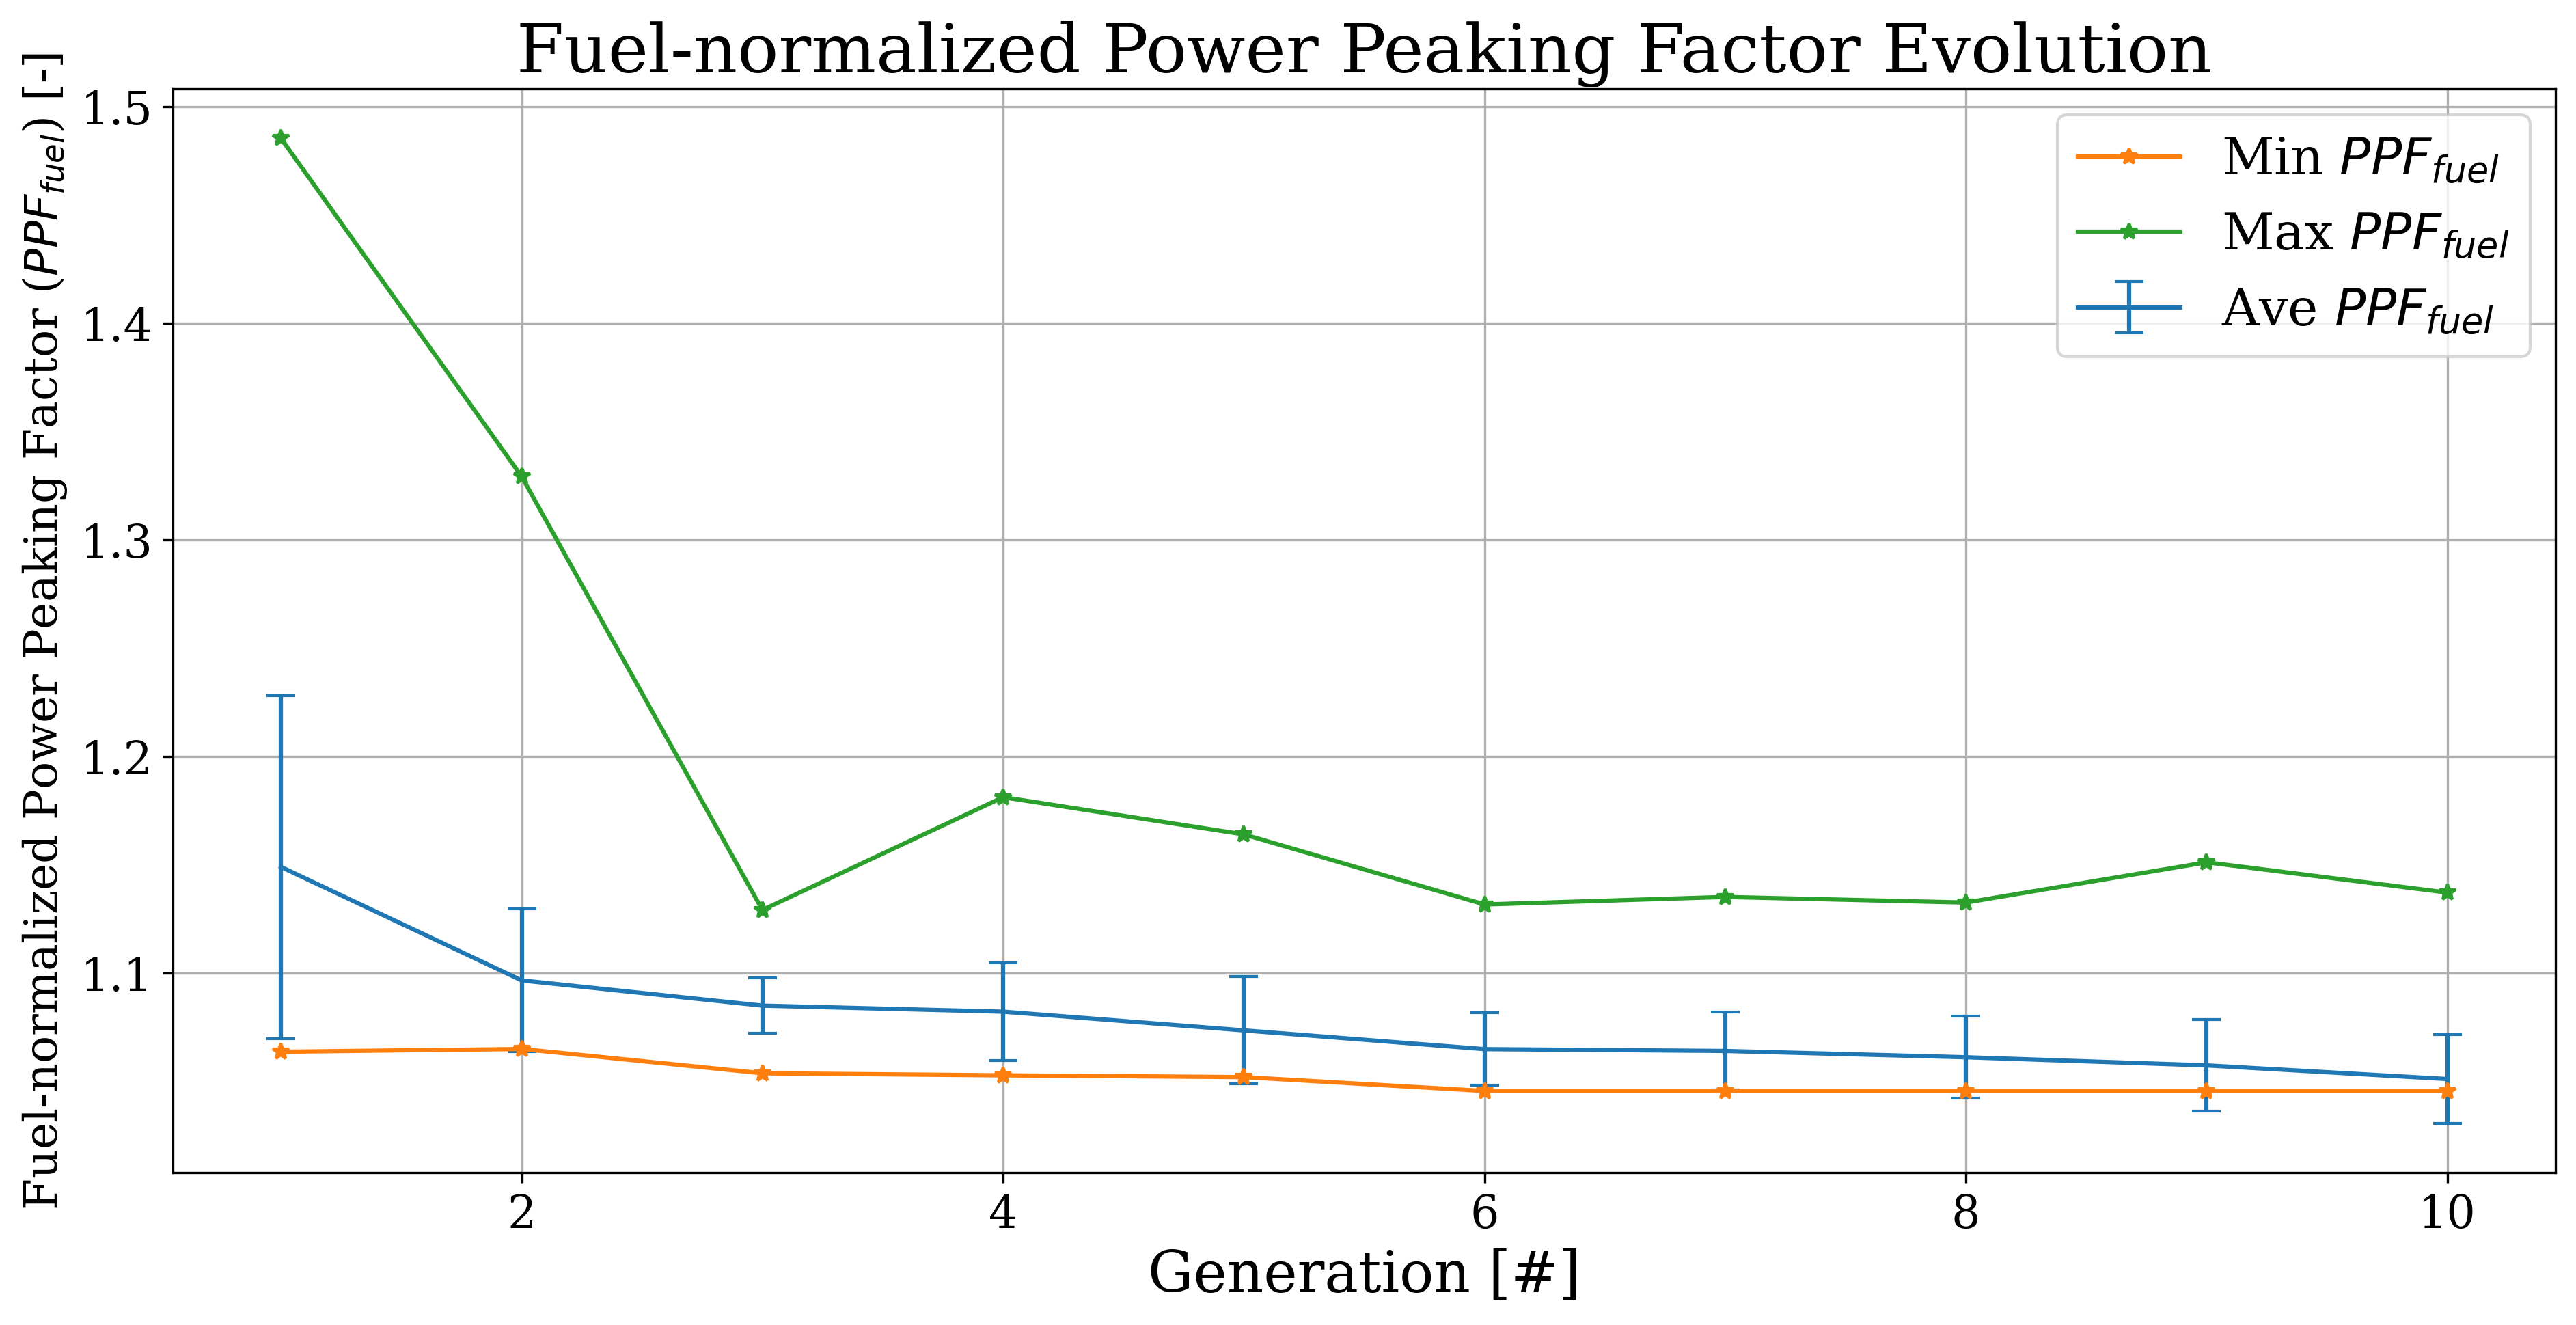
\includegraphics[width=\linewidth]{slab-obj-1-ppf-evol.png}
        \caption{Minimum, average, and maximum evolution of $PPF_{fuel}$ in the 
        AHTR plank.}
        \label{fig:slab-obj-1-ppf-evol} 
    \end{subfigure}
    \begin{subfigure}{0.9\textwidth}
        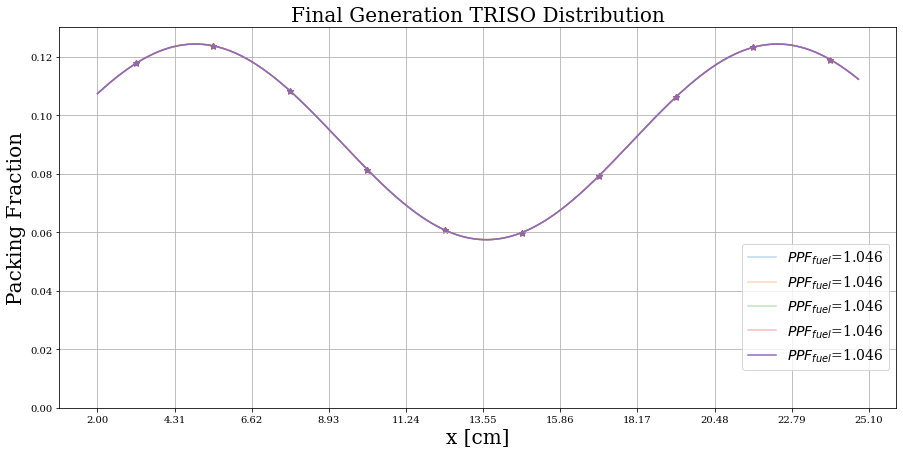
\includegraphics[width=\linewidth]{slab-obj-1-ppf-final.png}
        \caption{TRISO distribution for the 5 reactor models with the 
        lowest $PPF_{fuel}$ in AHTR plank at the final generation.}
        \label{fig:slab-obj-1-ppf-final} 
    \end{subfigure}
    \begin{subfigure}{0.9\textwidth}
        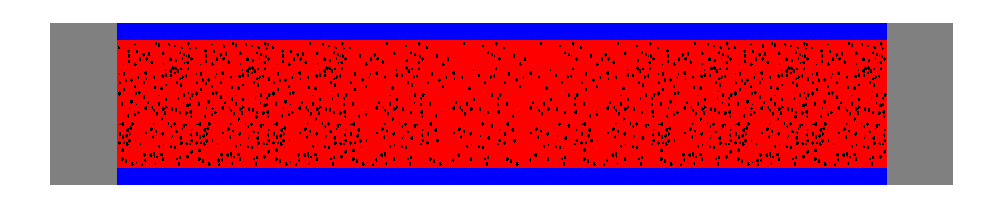
\includegraphics[width=\linewidth]{slab-obj-1-ppf-most-minimized.png}
        \caption{\gls{AHTR} plank model with most-minimized $PPF_{fuel}$
        (corresponds to the purple bolded distribution in the above plot).}
        \label{fig:slab-obj-1-ppf-most-minimized} 
    \end{subfigure}
    \caption{Simulation p-1c -- ROLLO single-objective optimization to minimize 
    AHTR plank's fuel-normalized power peaking factor ($PPF_{fuel}$). 
    Input parameters varied: TRISO distribution ($\rho_{TRISO}(\vec{r})$).
    $PF_{total}$ = 0.0979.}
    \label{fig:slab-obj-1-ppf}
\end{figure}

In Figure \ref{fig:slab-obj-1-ppf-final}, the TRISO distribution that best minimizes 
$PPF_{fuel}$ peaks near the edges of the fuel region of the plank, and has a minimum 
point in center of the plank.
This distribution is attributed to \gls{ROLLO} trying to flatten thermal flux in 
the plank to minimize fuel-normalized power peaking factor. 

Figure \ref{fig:flux-comparison-0.0979-plank} compares the flux distributions from the 
Figure \ref{fig:slab-obj-1-ppf-final}'s TRISO distribution and a constant 
$PF_{total}$ = 0.0979 TRISO distribution. 
\begin{figure}[htbp]
    \centering
    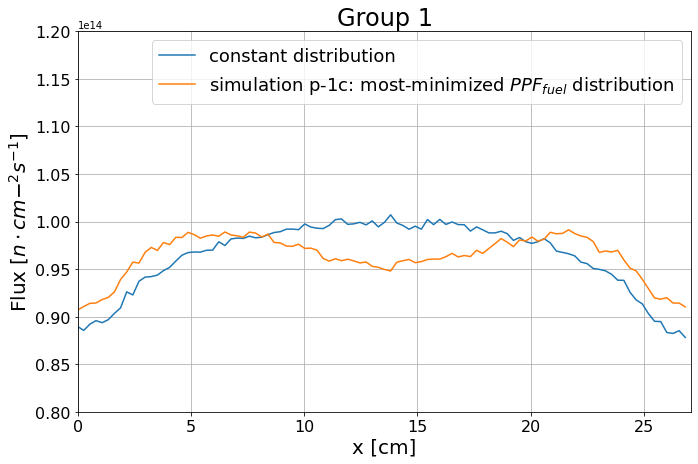
\includegraphics[width=0.48\linewidth]{flux-comparison-0.0979-plank_grp1.png} 
    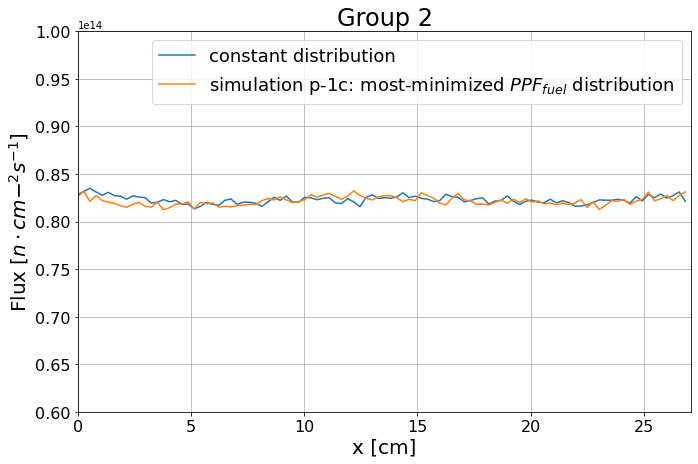
\includegraphics[width=0.48\linewidth]{flux-comparison-0.0979-plank_grp2.png} 
    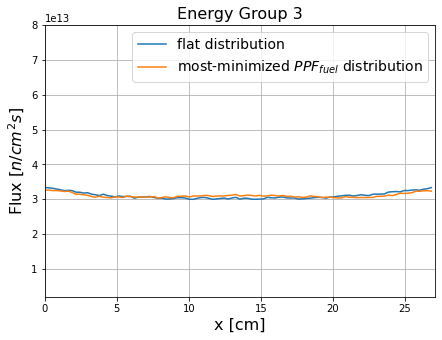
\includegraphics[width=0.48\linewidth]{flux-comparison-0.0979-plank_grp3.png} 
    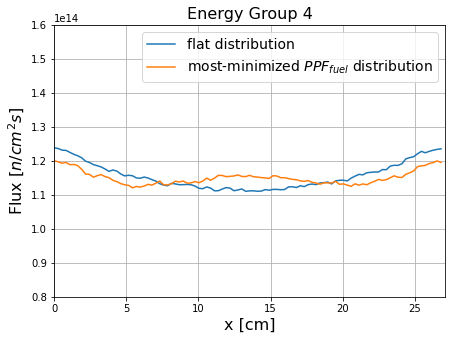
\includegraphics[width=0.48\linewidth]{flux-comparison-0.0979-plank_grp4.png} 
    \caption{Flux comparison between Figure \ref{fig:slab-obj-1-ppf-final}'s TRISO 
    distribution that most-minimized $PPF_{fuel}$ and a constant $PF_{total}$ = 0.0979 
    TRISO distribution. 
    \acrfull{AHTR} plank's centerline neutron flux distribution in 4 groups at 948K. 
    Centerline is the white line in Figure \ref{fig:ahtr-plank-verification}.
    Energy Group 1: E $> 9.1188 \times 10^{-3}$ MeV, 
    Energy Group 2: $2.9023 \times 10^{-5} < E < 9.1188 \times 10^{-3}$ MeV,
    Energy Group 3:  $1.8556 \times 10^{-5} < E < 2.9023 \times 10^{-5}$ MeV,
    Energy Group 4:  $1.0 \times 10^{-12} < E < 1.8554 \times 10^{-6}$ MeV.}
    \label{fig:flux-comparison-0.0979-plank}
\end{figure}
In Energy group 4, there most-minimized $PPF_{fuel}$ flux distribution is flatter than 
the constant $PF_{total}$ = 0.0979 flux distribution, resulting in a lower $PPF_{fuel}$. 
The dip in the constant $PF_{total}$ = 0.0979 thermal flux distribution is due to 
self-shielding effects. 

